\documentclass[
	10pt,								% globale Schriftgröße
	parskip=half-,						% setzt Absatzabstand hoch
	paper=a4,							% Format
	english,ngerman,					% lädt Sprachpakete
	]{scrartcl}							% Dokumentenklasse

% //////////////////// Pakete laden ////////////////////
\usepackage[fleqn]{amsmath}
\usepackage[fleqn]{mathtools}
\usepackage{amssymb}			% mathematische symbole, für \ceckmarks
\usepackage{amsthm}				% für proof
\usepackage{mathrsfs}			% für \mathscr
\usepackage{latexsym}
\usepackage{marvosym}				% für Lightning

\usepackage{fontspec} 			% funktioniert nur mit den neueren Compilern z.B. XeLaTeX
\usepackage{microtype}			% für bessere Worttrennung
\usepackage[ngerman]{babel} 	% Spracheinstellung
\usepackage{lmodern}			% verändert verwendete Schriftart, damit sie weniger pixelig ist

\usepackage{verbatim}
\usepackage{listings}			% Für Quellcode

\usepackage{graphicx}
\usepackage{tabularx}			% für Tabellen mit gleicher Spaltenbreite und automatischen Umbrüchen
\usepackage{fullpage}
\usepackage{multirow}			% für multirow in tabulars
\usepackage{rotate}
\usepackage[cmyk,table]{xcolor} % um Farben zu benutzen, kann mehr als das Paket color
\usepackage[					% Verlinkungen
	colorlinks,					% farbige Schrift, statt farbiger Rahmen
	linktocpage,				% verlinkt im Abb.Verzeichnis Seitenzahl statt Bildunterschrift
	linkcolor=blue				% setzt Farbe der Links auf blau
	]{hyperref}					% nur für digitale Anwendungen, url = "http://www.example.com"
\usepackage{url}				% für Webadressen wie e-mail usw.: "\url{http://www.example.com}"

\usepackage{enumerate}			% für versch. Aufzählungezeichen wie z.B. a)
\usepackage{xspace}				% folgt ein Leerzeichen nach einem \Befehl, wird es nicht verschluckt.
\usepackage{cancel}				% für das Durchstreichen u.a. in Matheformeln mit \cancel
\usepackage{float}              % zum Forcieren der Position von figure-Umgebungen

% zum Zeichnen (u.a. von Graphen)
\usepackage{fp}
\usepackage{tikz}
\usetikzlibrary{tikzmark}			% für \tikzmark{toRemember}
\usetikzlibrary{positioning}	% verbesserte Positionierung der Knoten
\usetikzlibrary{automata}		% für Automaten (GTI)
\usetikzlibrary{arrows}
\usetikzlibrary{shapes}
\usetikzlibrary{decorations.pathmorphing}
\usetikzlibrary{decorations.pathreplacing}
\usetikzlibrary{decorations.shapes}
\usetikzlibrary{decorations.text}

% //////////////////// Syntaxhighlighting ////////////////////
\lstloadlanguages{Python, Haskell, [LaTeX]TeX, Java}
\lstset{
   basicstyle=\footnotesize\ttfamily,	% \scriptsize the size of the fonts that are used for the code
   backgroundcolor = \color{bgcolour},	% legt Farbe der Box fest
   breakatwhitespace=false,	% sets if automatic breaks should only happen at whitespace
   breaklines=true,			% sets automatic line breaking
   captionpos=t,				% sets the caption-position to bottom, t for top
   commentstyle=\color{codeblue}\ttfamily,% comment style
   frame=single,				% adds a frame around the code
   keepspaces=true,			% keeps spaces in text, useful for keeping indentation
							% of code (possibly needs columns=flexible)
   keywordstyle=\bfseries\ttfamily\color{codepurple},% keyword style
   numbers=left,				% where to put the line-numbers;
   							% possible values are (none, left, right)
   numberstyle=\tiny\color{codegreen},	% the style that is used for the line-numbers
   numbersep=5pt,			% how far the line-numbers are from the code
   stepnumber=1,				% nummeriert nur jede i-te Zeile
   showspaces=false,			% show spaces everywhere adding particular underscores;
							% it overrides 'showstringspaces'
   showstringspaces=false,	% underline spaces within strings only
   showtabs=false,			% show tabs within strings adding particular underscores
   flexiblecolumns=false,
   tabsize=1,				% the step between two line-numbers. If 1: each line will be numbered
   stringstyle=\color{orange}\ttfamily,	% string literal style
   numberblanklines=false,				% leere Zeilen werden nicht mitnummeriert
   xleftmargin=1.2em,					% Abstand zum linken Layoutrand
   xrightmargin=0.4em,					% Abstand zum rechten Layoutrand
   aboveskip=2ex, 
}

\lstdefinestyle{py}{
   language=Python,
}
\lstdefinestyle{hs}{
   language=Haskell,
}
\lstdefinestyle{tex}{
	language=[LaTeX]TeX,
	escapeinside={\%*}{*)},     % if you want to add LaTeX within your code
	texcsstyle=*\bfseries\color{blue},% hervorhebung der tex-Schlüsselwörter
	morekeywords={*,$,\{,\},\[,\],lstinputlisting,includegraphics,
	rowcolor,columncolor,listoffigures,lstlistoflistings,
	subsection,subsubsection,textcolor,tableofcontents,colorbox,
	fcolorbox,definecolor,cellcolor,url,linktocpage,subtitle,
	subject,maketitle,usetikzlibrary,node,path,addbibresource,
	printbibliography},% if you want to add more keywords to the set
     numbers=none,
     numbersep=0pt,
     xleftmargin=0.4em,
}

\lstdefinestyle{java}{
	language=Java,
	extendedchars=true,		% lets you use non-ASCII characters;
   						% for 8-bits encodings only, does not work with UTF-8
}

\lstdefinelanguage[x64]{Assembler}     % add a "x64" dialect of Assembler
   [x86masm]{Assembler} % based on the "x86masm" dialect
   % with these extra keywords:
   {morekeywords={CDQE,CQO,CMPSQ,CMPXCHG16B,JRCXZ,LODSQ,MOVSXD, %
                  POPFQ,PUSHFQ,SCASQ,STOSQ,IRETQ,RDTSCP,SWAPGS, %
                  rax,rdx,rcx,rbx,rsi,rdi,rsp,rbp, %
                  r8,r8d,r8w,r8b,r9,r9d,r9w,r9b}
}					% for 8-bits encodings only, does not work with UTF-8

\lstdefinestyle{c}{
	language=c,
	extendedchars=true,		% for 8-bits encodings only, does not work with UTF-8
}

% //////////////////// eigene Kommandos ////////////////////
\newcommand\FU{Freie Universität Berlin\xspace}% benötigt package xspace
\newcommand\gdw{g.\,d.\,w.\xspace}
\newcommand\oBdA{o.\,B.\,d.\,A.\xspace}
\newcommand{\Eu}{\texteuro}
\newcommand\N{\mathbb{N}\xspace}
\newcommand\Q{\mathbb{Q}\xspace}
\newcommand\R{\mathbb{R}\xspace}
\newcommand\Z{\mathbb{Z}\xspace}
\newcommand\ohneNull{\ensuremath{\backslash\lbrace 0\rbrace}}% \{0}
\let\dhALT\dh	% Schreibt Befehl \dh in \dhALT um
\renewcommand\dh{d.\,h.\xspace}	%renew überschreibt command \dh
\newcommand\Bolt{\;\text{\LARGE\raisebox{-0.3em}{\Lightning}\normalsize}\xspace}% Blitz
\newcommand\zz{\ensuremath{\raisebox{+0.25ex}{Z}% zu zeigen
			\kern-0.4em\raisebox{-0.25ex}{Z}%
			\;\xspace}}
\newcommand{\from}{\ensuremath{\colon}}
\newcommand{\floor}[1]{\lfloor{#1}\rfloor}
\newcommand{\ceil}[1]{\lceil{#1}\rceil}
 \renewcommand{\L}{\ensuremath{\mathcal{L}}\xspace}
 \renewcommand{\P}{\ensuremath{\mathcal{P}}\xspace}
 \newcommand{\NL}{\ensuremath{\mathcal{N}\kern-0.2em\mathcal{L}}\xspace}
 \newcommand{\NP}{\ensuremath{\mathcal{NP}}\xspace}

% //////////////////// Mathefunktionen ////////////////////
\DeclareMathOperator{\Landau}{\mathcal{O}}
\DeclareMathOperator{\True}{True}
\DeclareMathOperator{\False}{False}

% //////////////////// eigene Theoreme ////////////////////
\newtheorem{theorem}{Satz}
\newtheorem{corollary}[theorem]{Folgerung}
\newtheorem{lemma}[theorem]{Lemma}
\newtheorem{observation}[theorem]{Beobachtung}
\newtheorem{definition}[theorem]{Definition}
\newtheorem{Literatur}[theorem]{Literatur}
% konfiguriert proof
\makeatletter
\newenvironment{Proof}[1][\proofname]{\par
  \pushQED{\qed}%
  \normalfont \topsep6\p@\@plus6\p@\relax
  \trivlist
  \item[\hskip\labelsep
%         \itshape
        \bfseries
    #1\@addpunct{.}]\ignorespaces
}{%
  \popQED\endtrivlist\@endpefalse
}
\makeatother

% //////////////////// eigene Farben ////////////////////
\let\definecolor=\xdefinecolor
\definecolor{FUgreen}{RGB}{153,204,0}
\definecolor{FUblue}{RGB}{0,51,102}

\definecolor{middlegray}{rgb}{0.5,0.5,0.5}
\definecolor{lightgray}{rgb}{0.8,0.8,0.8}
\definecolor{orange}{rgb}{0.8,0.3,0.3}
\definecolor{azur}{rgb}{0,0.7,1}
\definecolor{yac}{rgb}{0.6,0.6,0.1}
\definecolor{Pink}{rgb}{1,0,0.6}

\definecolor{bgcolour}{rgb}{0.97,0.97,0.97}
\definecolor{codegreen}{rgb}{0,0.6,0}
\definecolor{codegray}{rgb}{0.35,0.35,0.35}
\definecolor{codepurple}{rgb}{0.58,0,0.82}
\definecolor{codeblue}{rgb}{0.4,0.5,1}

% //////////////////// eigene Settings ////////////////////

\textheight = 230mm		% Höhe des Satzspiegels / Layouts
\footskip = 10ex			% Abstand zw. Fußzeile und Grundlinie letzter Textzeile
\parindent 0pt			% verhindert Einrückung der 1. Zeile eines Absatzes
\setkomafont{sectioning}{\rmfamily\bfseries}% setzt Ü-Schriften in Serifen, {disposition}											% bindet Header ein (WICHTIG)
\usepackage{graphicx}
\usepackage{fancyvrb}

\newcommand{\dozent}{Prof. Dr. Agn`es Voisard, Nicolas Lehmann}					% <-- Names des Dozenten eintragen
\newcommand{\tutor}{Nicolas Lehmann}						% <-- Name eurer Tutoriun eintragen
\newcommand{\tutoriumNo}{10}				% <-- Nummer im KVV nachschauen
\newcommand{\projectNo}{2}									% <-- Nummer des Übungszettels
\newcommand{\veranstaltung}{Datenbanksysteme}	% <-- Name der Lehrveranstaltung eintragen
\newcommand{\semester}{SoSe 2017}						% <-- z.B. SoSe 17, WiSe 17/18
\newcommand{\studenten}{Boyan Hristov, Julian Habib}			% <-- Hier eure Namen eintragen
% /////////////////////// BEGIN DOKUMENT /////////////////////////


\begin{document}
% /////////////////////// BEGIN TITLEPAGE /////////////////////////
\begin{titlepage}
	\subject{\dozent}
	\title{\veranstaltung, \semester}
	\subtitle{\Large Übungsblatt \projectNo\\ \large\vspace{1ex} TutorIn: \tutor\\ Tutorium \tutoriumNo}
	\author{\studenten}
	\date{\normalsize \today}
\end{titlepage}

\maketitle								% Erstellt das Titelblatt
\vspace*{-10cm}							% rückt Logo an den oberen Seitenrand
\makebox[\dimexpr\textwidth+1cm][r]{	%rechtsbündig und geht rechts 1cm über Layout hinaus
	
\includegraphics[width=0.4\textwidth]{src/fu_logo} % fügt FU-Logo ein
}
% /////////////////////// END TITLEPAGE /////////////////////////

\vspace{7cm}							% Abstand
\rule{\linewidth}{0.8pt}				% horizontale Linie										% erstellt die Titelseite


Link zum Git Repository: \url{https://github.com/BoyanH/Freie-Universitaet-Berlin/tree/master/Datenbanksysteme/Solutions/homework3}

% /////////////////////// Aufgabe 1 /////////////////////////
\section{Aufgabe}


\begin{itemize}

\item[a)]

Relationales Modell \\

% Relational Modell
\begin{Verbatim}[commandchars=+\[\]]

Person(+underline[ID::integer], Age::integer, Name::character varying(20), Password::character varying(40),
	Login::character varying(40))
Teacher(+underline[ID::integer])
Student(+underline[ID::integer])
Course(+underline[Number::integer], Name :: character varying(50))
Module(+underline[Number::integer], Name :: character varying(50))

PersonIsATeacher(+underline[PersonID, TeacherID])
PersonIsAStudent(+underline[PersonID, StudentID])
TeachesCourses(+underline[PersonID, CourseNumber], InSemester)
ContainsCourses(+underline[ModuleNumber, CourseNumber])
AttendsCourses(+underline[StudentID, CourseNumber])
\end{Verbatim}
% End of relational Modell

ER Diagramm in umgekehrter min-max Chen Notation \\

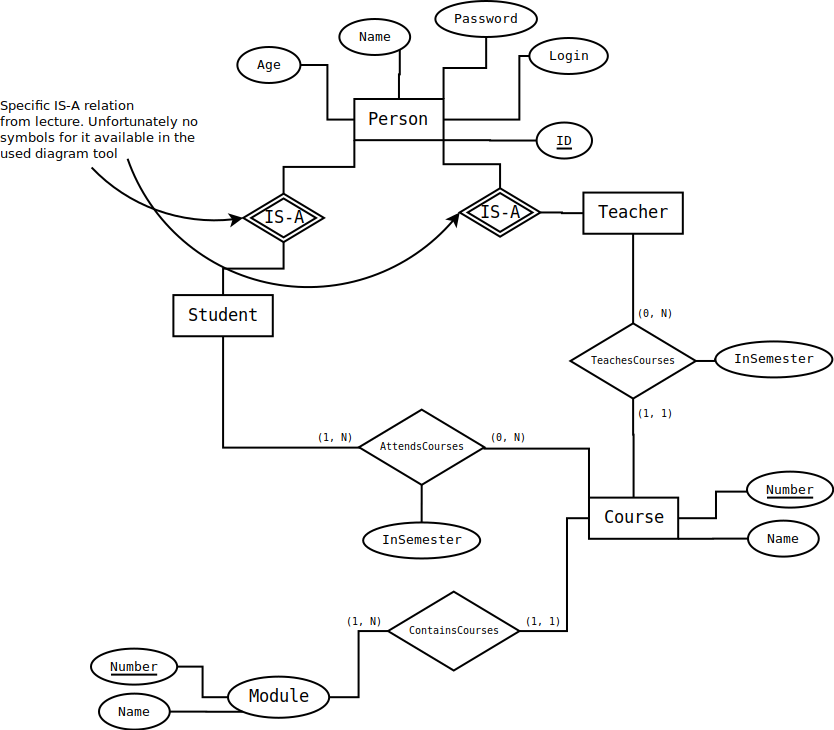
\includegraphics[width=\textwidth]{./src/exercise3_A.png}


\item[b)] 

Relationales Modell \\

% Relational Modell
\begin{Verbatim}[commandchars=+\[\]]

Person(+underline[ID::integer], Name::character varying(20))
Doctor(+underline[ID::integer], Specialty::character varying(30), Name::character varying(20))
Patient(+underline[ID::integer], HealthHistory::character varying(40) ARRAY, Name::character varying(20))
DoctorsAppointment(+underline[ID::integer], Date::date)
Address(+underline[PrivateAddressStreet::character varying(20)], City::character varying(20), 
	ServiceAddressStreet::character varying(20))

LivesIn(+underline[PersonID, AddressPrivateAdressStreet])
Attends(+underline[PersonID, DoctorsAppointmentID])
Services(+underline[PersonID, DoctorsAppointmentID])
\end{Verbatim}
% End of relational Modell

ER Diagramm in umgekehrter min-max Chen Notation\\

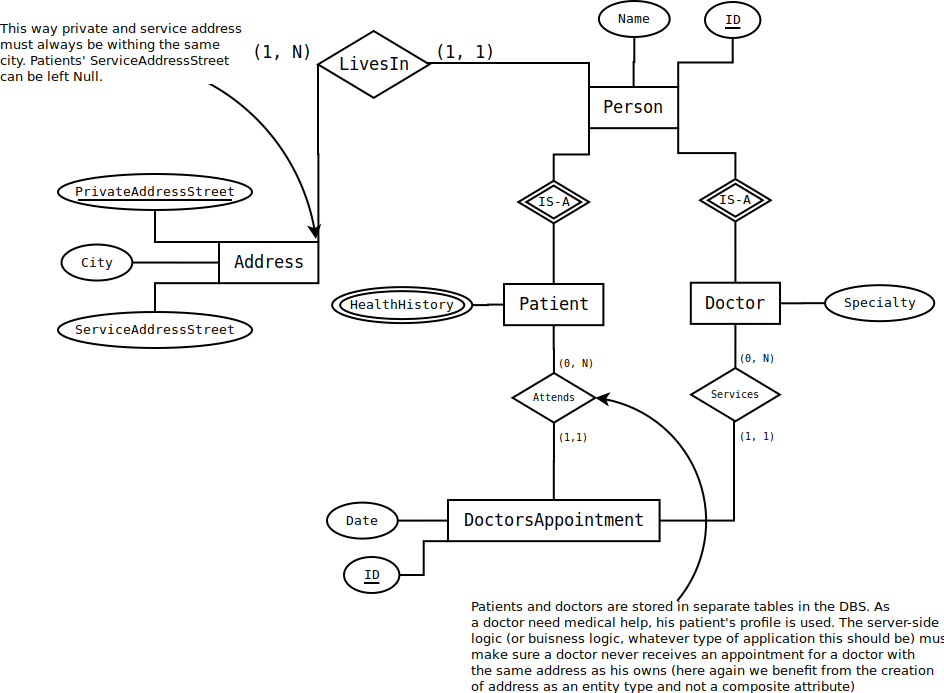
\includegraphics[width=\textwidth]{./src/exercise3_B.png}

\end{itemize}

\section{Aufgabe}

\begin{itemize}


\item[a)]
$\Pi_{\text{Vorname, Nachname}}$ ($\sigma_{\text{Alter} < 30 }$)

\item[b)]
$\Pi_{\text{Datum}}$ ($\sigma_{\text{Temperatur > Regenmenge } \lor \text{ Temperatur > Sonnenscheindauer} }$)

\item[c)]
$\Pi_{\text{Kreditkartennummer}}$ ($\sigma_{\text{Name = 'Emirates' $\land$ Datum $\geq$ '02.03.2016' $\land$ Datum $\leq$ '07.06.2016'}}$  (Passagier $\bowtie_{\text{ID = Passagier-ID}}$ Flug $\bowtie_{\text{Fluggesellschaft-ID = ID}}$ Fluggesellschaft))

\item[d)]
$\Pi_{\text{Name}}$ ($\sigma_{\text{Temperatur < 0}}$ (Wetter $\bowtie_{\text{Wetter::Datum = Flug::Datum}}$ Flug $\bowtie_{\text{Fluggesellschaft-ID = ID}}$ Fluggesellschaft))

\item[e)]
$\Pi_{\text{Vorname, Nachname}}$ ($\sigma_{\neg\text{(Temperatur < 20 $\land$ Regenmenge > 10 $\land$ Sonnenscheindauer < 6)}}$ (Wetter $\bowtie_{\text{Wetter::Datum = Flug::Datum}}$ Flug $\bowtie_{\text{Passagier-ID = ID}}$ Passagier))

\end{itemize}

\section{Aufgabe}

Um die Aufgabe richtig zu lösen, muss man Attribute (Spalten) umbenennen können. Sonst kann man nicht äußern, dass z.B. Nachname und Datum gleich sein müssen, ID aber nicht. 
Nach der Annahme, dass wir die Operation zum Umbenennen benutzen können, kann man die Folgende aufgaben so lösen (Diese Operation ist offiziel in der relationalen Algebra enthalten). \\

Wir haben die einzelne Teile in separate Queries geteilt, damit man besser verstehen kann was genau passiert.

\begin{itemize}

\item[a)]

q1 = $\sigma_{text{Alter > 30}}$ (Passagier $\bowtie_{\text{ID = Passagier-ID}}$ Flug) \\
q2 = $\Pi_{\text{Vorname, Nachname, Datum, Fluggesellschaft-ID}}$ (q1) \\
q3 = q2 $\bowtie (\delta$ 'Vorname' $\rightarrow$ 'Vorname-duplicate' q2) \\
q4 = q3 - $\sigma_{\text{Vorname = Vorname-duplicate}} (q3)$ \\
q5 = $\Pi_{\text{Vorname, Nachname}}$ (q4) \\

q1 nimmt alle Passagiere, die über 30 Jahre alt sind und die dazugehörige Fluge.
q2 nimmt nur die Attributen Vorname, Nachname, Datum und Fluggesellschaft-ID davon. Dies wird gemacht, damit dann bei q3 alle mögliche Kombinationen von Passagieren, die im selben Flug geflogen sind und die selbe Nachname haben (wir haben angenommen, das ein Flug durch Datum und Fluggesellschaft-ID eindeutig charakterisiert wird) erzeugt werden. Dann sorgt q4 dass Entitäten mit gleiche Vorname und Vorname-duplicate gelöscht werden. Fall mindestends 2 Personen mit dem selben Nachname gibt, dann gibt es mindestens 4 Entitäten, die originelle und diese mit vertauschte Vorname und Vorname-duplicate. Nur diese mit vertauschte (unterschiedliche) Vorname und Vorname-duplicate werden im q4 selektiert. Danach wird in q5 die Vorname und Nachname dieser Entitäten selektiert.

\item[b)]

q1 = Passagier $\bowtie_{\text{ID = Passagier-ID}}$ Flug \\
q2 = $\Pi_{\text{Alter, Datum, Fluggesellschaft-ID}}$ (q1) \\
q3 = q2 $\bowtie (\delta$ 'Alter' $\rightarrow$ 'Alter-duplicate' q2) \\
q4 = q2 - $\sigma_{\text{Alter = Alter-duplicate}}$ (q2) \\
q5 = $\Pi_{\text{Datum, Fluggesellschaft-ID}}$ (q4) \\
q6 = q1 - q5 \\
q7 = $\Pi_{\text{Datum, Fluggesellschaftsname}}$ (q6 $\bowtie_{\text{FluggesellschaftID = ID}}$ Fluggesellschaft) \\

Nach der selben Logik haben wir in q4 Alle Flüge, auf dem mindestens zwei Personen das selbe Alter haben. In q5 nehmen wir nur Datum und Fulggesellschaft-ID (Das Superkey einer Flug, nach Annahme) damit wir in q6 alle Flüge bekommen können, die nur Passagiere mit verschiedenem Alter haben. Dann wird in q7 die Fluggesellschaft Tabelle dazugenommen, damit Datum und Fluggesellschaftsname zurückgegeben werden können. \\ \\

Quelle - eine analoge Frage im StackOverflow: \url{https://stackoverflow.com/questions/43567351/relational-algebra-natural-join-of-table-q2-with-rename-of-table-q2-for-passenge}

\section{Aufgabe}

\begin{lstlisting}

<!DOCTYPE html>
<html>
<head>
	<meta charset="utf-8"></meta>
	<title>Apple Aktie</title>
	<style type="text/css">

		#linechart, #barchart {

			width: 600px;
			height: 400px;
		}

	</style>
	<script type="text/javascript" language="javascript" src="./bower_components/jquery/dist/jquery.min.js"></script>
	<script type="text/javascript" language="javascript" src="./bower_components/Flot/jquery.flot.js"></script>
</head>
<body>
	<div id="linechart"></div>
	<div id="barchart"></div>
	<script type="text/javascript">

		function parseDataToObject(data) {

			var rows = data.split('\r\n').map(function (item) {
				return item.replace(';', '').split(',');
			});
			var attributes = rows[0];
			var parsedObject = {};

			rows = rows.slice(1);
			attributes.forEach(function (attr, idx) {

				parsedObject[attr] = rows.map(function (row) {
					
					if(attr === 'Datum') {
				
						var crntDate = new Date(),
							crntDecade = crntDate.getFullYear().toString().slice(0,2);
							valueArr = row[idx].split('.'),
							day = valueArr[0]*1,
							month = valueArr[1]*1 - 1,
							year = (crntDecade + valueArr[2])*1,
							date = new Date(year, month, day);

						return date.getDate()*1;
					}
					return row[idx]*1;
				});
			});

			return parsedObject;
		}

		function mergeArrayEntities(arrA, arrB) {

			var copyA = arrA.slice(0),
				copyB = arrB.slice(0);

			if(copyA.length !== copyB.length) {

				throw new Error('Only arrays with equal length can be merged!');
			}

			return copyA.map(function (item, idx) {

				return [item, copyB[idx]];
			});
		}

		$.get('./data/apple.csv', function(data) {

			var parsedData = parseDataToObject(data);
			
			$.plot($('#linechart'), 
				[

					{color: '#f00', data: mergeArrayEntities(parsedData.Datum, parsedData.Tief)},
					{color: '#0f0', data: mergeArrayEntities(parsedData.Datum, parsedData.Hoch)},
					{color: '#ff0', data: mergeArrayEntities(parsedData.Datum, parsedData.Tagesendwert)}

			]);

			$.plot($('#barchart'), 
				[

					{color: '#f00', data: mergeArrayEntities(parsedData.Datum, parsedData.Handelsvolumen)}

				], 
				{
		            series: {
		                bars: {
		                    show: true
		                }
		            },
		            bars: {
		                align: "center",
		                barWidth: 0.5
		            }
			});

		});

	</script>
</body>
</html>

\end{lstlisting}


\end{itemize}




% /////////////////////// END DOKUMENT /////////////////////////
\end{document}